%%%%%%%%%%%%%%%%%%%%%%%%%%%%%%%%%%%%%%%%%%%%%%%%%%%%%%%%%%%%%%%%%%%%%%%%
%
% First comes an example EPS file -- just ignore it and
% proceed on the \documentclass line
% your LaTeX will extract the file if required
\begin{filecontents*}{example.eps}
%!PS-Adobe-3.0 EPSF-3.0
%%BoundingBox: 19 19 221 221
%%CreationDate: Mon Sep 29 1997
%%Creator: programmed by hand (JK)
%%EndComments
gsave
newpath
  20 20 moveto
  20 220 lineto
  220 220 lineto
  220 20 lineto
closepath
2 setlinewidth
gsave
  .4 setgray fill
grestore
stroke
grestore
\end{filecontents*}
%
\RequirePackage{fix-cm}
%
%\documentclass{svjour3}                     % onecolumn (standard format)
%\documentclass[smallcondensed]{svjour3}     % onecolumn (ditto)
\documentclass[smallextended]{svjour3}       % onecolumn (second format)
%\documentclass[twocolumn]{svjour3}          % twocolumn
%
\smartqed  % flush right qed marks, e.g. at end of proof
%
% \usepackage{mathptmx}      % use Times fonts if available on your TeX system
%
% insert here the call for the packages your document requires
%\usepackage{latexsym}
% etc.
%
\usepackage{graphicx}
\usepackage[round]{natbib}
\usepackage{amssymb,amsmath}
%
% please place your own definitions here and don't use \def but
\newcommand{\mnras}{MNRAS}
\newcommand{\nat}{Nature}
\newcommand{\aap}{A\&A}
\newcommand{\apj}{ApJ}
\newcommand{\aj}{AJ}
\newcommand{\apjl}{ApJL}
\newcommand{\apjs}{ApJS}
\newcommand{\jcap}{JCAP}
\newcommand{\physrep}{Phys.Rep.}
\newcommand{\prd}{Phys.Rev.D}
\newcommand{\araa}{ARA\&A}
\newcommand{\Ddt}{D_{\Delta{\rm t}}}
\newcommand{\Dd}{D_{\rm d}}
\newcommand{\Ds}{D_{\rm s}}
\newcommand{\Dds}{D_{\rm ds}}
\newcommand{\zd}{z_{\rm d}}
\newcommand{\zs}{z_{\rm s}}
\newcommand{\cospars}{\boldsymbol{\Omega}}
\newcommand{\Ok}{\Omega_{\rm k}}
\newcommand{\ODE}{\Omega_{\rm DE}}
\newcommand{\wDE}{w_0}
\newcommand{\x}{\boldsymbol{\theta}}
\newcommand{\y}{\boldsymbol{\beta}}
\newcommand{\grad}{\boldsymbol{\nabla}}
\newcommand{\deflectionangle}{\boldsymbol{\alpha}}
%
% Insert the name of "your journal" with
% \journalname{myjournal}
%
%%%%%%%%%%%%%%%%%%%%%%%%%%%%%%%%%%%%%%%%%%%%%%%%%%%%%%%%%%%%%%%%%%%%%%%%

\begin{document}

\title{Time Delay Cosmography%\thanks{Grants or other notes
%about the article that should go on the front page should be
%placed here. General acknowledgments should be placed at the end of the article.}
}
%\subtitle{Time delay cosmography}

\titlerunning{Time Delay Cosmography}        % if too long for running head

\author{Tommaso Treu         \and
        Philip J. Marshall %etc.
}

%\authorrunning{Treu \& Marshall} % if too long for running head

\institute{Tommaso~Treu \at
Department of Physics and Astronomy, \\
University of California,\\
Los Angeles, CA 90095, USA\\
\email{tt@astro.ucla.edu}           %  \\
%             \emph{Present address:} of F. Author  %  if needed
           \and
Philip~J.~Marshall \at
Kavli Institute for Particle Astrophysics and Cosmology, \\
P.O. Box 20450, MS29, \\
Stanford, CA 94309, USA \\
}

\date{Received: date / Accepted: date}
% The correct dates will be entered by the editor

\maketitle

%%%%%%%%%%%%%%%%%%%%%%%%%%%%%%%%%%%%%%%%%%%%%%%%%%%%%%%%%%%%%%%%%%%%%%%%

\begin{abstract}

Gravitational time delays, observed in strong lens systems where the
variable background source is multiply-imaged by a massive galaxy in
the foreground, provide direct measurements of cosmological distance
that are very complementary to other cosmographic probes. The success
of the technique depends on the availability and size of a suitable
sample of lensed quasars or supernovae, precise measurements of the
time delays, accurate modeling of the gravitational potential of the
main deflector, and our ability to characterize the distribution of
mass along the line of sight to the source. We review the progress
made during the last 15 years, during which the first competitive
cosmological inferences with time delays were made, and look ahead to
the potential of significantly larger lens samples in the near future.
\keywords{cosmology, gravitational lensing, gravity, dark energy}
% \PACS{PACS code1 \and PACS code2 \and more}
% \subclass{MSC code1 \and MSC code2 \and more}

\end{abstract}

%%%%%%%%%%%%%%%%%%%%%%%%%%%%%%%%%%%%%%%%%%%%%%%%%%%%%%%%%%%%%%%%%%%%%%%%

\section{Introduction}
\label{sec:intro}

The measurement of cosmic distances is central to our understanding of
cosmography, i.e. the description of the geometry and kinematics of
the universe. The discovery of the period luminosity relation for
cepheids led to the realization that the universe is much bigger than
the Milky Way and that it is currently expanding. Relative distance
measurements based on supernova Ia light curves were the turning point
in the discovery of the acceleration of the universe
\citep{Riess:1998p21184,Per++99}.

In the two decades since the discovery of the acceleration of the
universe, distance measurements have improved steadily. For example,
the Hubble constant has now been measured to 3\% precision
\citep{Rie++11,Fre++12}
while the distance to the last scattering surface of the cosmic
microwave backgrond is now known to better than 1\% precision
\cite{WMAP9,Planck15}. This precision is more than sufficient for all purposes
related to our understanding of phenomena occurring within the
universe, like galaxy evolution.

In spite of all this progress, the most fundamental question still
remains unanswered. What is causing the acceleration? Is this {\it
dark energy} something akin to Einstein's cosmological constant or is
it a dynamical component? Answering this question from an empirical
standpoint will require further improvements in the precision of
distance measurements \citep{Wei++13}.  [EXPLAIN DEGENERACY IN CMB
DATA AND NEED FOR LOWER REDSHIFT PROBES]

Many dedicated experiments are currently under way or being planned
with ths goal in mind.

Precision, however, is not sufficient by itself. In addition to
controlling the known statistical uncertainties, modern day
experiments need to control stystematic errors in order to fullfill
their potential, including the infamous unknow unknowns. The most
direct way to demonstrate {\it accuracy} is to compare independent
measurements with comparable {\it precision}. [MENTION LITTLE TENSION
BETWEEN WMAP9 AND PLANCK: MAKE PLOT SHOWING H0 LOCALLY VS H0 FROM CMB?]

Ideally, the comparison between independent measurements should be
carried out blindly, so as to minimize experimenter bias. Two blind
mutually blind measurements agreeing that the equation of state
parameter $w$ is not $-1$ would be a very convincing demonstration
that the dark energy is not the cosmological constant. Conversely, the
significant disagreement of two independent measurements, could open
the door to the discovery of new physics.

In this review we focus on gravitational time delay as a tool for
cosmography.  Gravitational time delays are a natural phenomenon in
general relativity and provide a direct and elegant way to measure
absolute distances out to cosmological redshift. When the line of
sight to a distant source of light is suitably well aligned with an
intervening massive system, multiple images appear to the
observer. The arrival time of the images depends on the interplay of
the geometric and gravitational delays specific to the
configuration. If the emission from the source is variable in time,
the difference in arrival time is measurable, and can be converted
into the so-called time delay distance $\Ddt$, a combination of
angular diameter distances to the deflector and source. $\Ddt$ is
inversely proportional to the Hubble Constant $H_0$ and it is more
weakly dependent on other cosmological parameters. The sensitivity to
$H_0$ and independence to the local distance ladder method make time
delays a very valuable cosmological tool for precise and accurate
cosmology. [EXPLAIN MORE IN DETAIL INDEPENDENCE OF DISTANCE LADDER AND
TD] As several authors have pointed out
\citep{Lin11,Suy++12,Wei++13}, achieving sub-percent precision and
accuracy on the measurement of the Hubble constant is a powerful
addition to stage III and IV dark energy experiments.

This review is organized as follows. In Section~\ref{sec:intro} we
summarize the history of time delay cosmography up until the turn of
the millennium, in order to give a sense of the early challenges and
how they were overcome. In Section~\ref{sec:theory}, we review the
theoretical foundations of the method, in terms of the gravitational
optics version of Fermat's principle. In Section~\ref{sec:measurement}
we describe in some detail the elements of a modern time delay
distance measurement, emphasizing recent advances and remaining
challenges. In Section~\ref{sec:cosmo} we elucidate the connection
between time delay distance measurements and cosmological parameters,
discussing complementarity with other cosmological
probes. Section~\ref{sec:outlook} critically examines the future of
the method, discussing prospects for increasing the precision, testing
for accuracy, and synergy with other future probes of dark energy. A
brief summary is given in Section~\ref{sec:summary}. Owing to space
limitations, we could only present a selection of all the beautiful
work that has been published on this topic in the past decades. We
refer the readers to recent
\citep{Bar10,Ell10,Tre10,TMC12,Jackson:2013p30763,Jac15,T+E15} and not-so-recent \citep{B+N92,CSS02,K+S04,Fal05,SKW06}
excellent reviews and textbooks \citep{SEF92} for additional
information and historical context.

%xCite Jackson 2015, Weinberg 2013, etc etc.


%%%%%%%%%%%%%%%%%%%%%%%%%%%%%%%%%%%%%%%%%%%%%%%%%%%%%%%%%%%%%%%%%%%%%%%%

\section{A brief history of time delay cosmography}
\label{sec:history}

\citet{Ref64} first suggested that strong lens time delays could be
used to measure absolute distances out to cosmological distances, and
therefore the Hubble Constant to leading order. Unfortunately, no
strong lensing systems were known at that time, and therefore his
intuition remained purely theoretical for over a decade.

The prospects of using time delays for cosmography suddenly brightened
in the late seventies, with the discovery of the first strongly lensed
quasars \citep{WCW79}. Even though they were not the strongly lensed
supernovae that Refsdal had in mind, quasars fluxes are sufficiently
variable \citep{Van82} that people were able to start to put Refsdal's
idea in practice \citep{Van89}. For completeness, we should mention
that the first multiply imaged supernova has been discovered in 2014,
fifty years afer Refsdal's initial suggestion \citep{Kel++15}, lensed
by a foreground cluster of galaxies. The time delays are being
measured at the time of writing
\citep{Rod++16,Kel++16}. However, it is unclear at the moment whether the
cluster potential can be constrained with sufficient precision to
yield interesting cosmological information \citep{Tre++16}. Therefore,
in this review, we will restrict our case to the much more common and
better understood case of a variable quasar being lensed by a
foreground elliptical galaxy.

Discovery and monitoring of lensed quasars continued in the eighties and
nineties, powered by heroic efforts. By the end of the millennium the
number of known strongly lensed systems was in double digits
\citep{CSS02}, and the first truly robust time delays were measured
\citep{Kun++97,Sch++97}.

The discovery of multiply imaged quasars finally took off at the
beginning of the current Millennium with the improvement of panoramic
search technology in dedicated or existing surveys
\citep{Bro++03,Oguri:2006p5865,Agn++15}.

The period of time delay cosmography was marred by controversies over
systematic errors.  The measurement of time delays was particularly
controversial during the nineties as the quality of the early data
allowed for multiple values \citep{PRH92}, owing to the combined
effects of gaps in the data, and microlensing noise in the optical
light curves. This problem was definitely solved at the turn of the
millennium, with the beginning of modern monitoring campaigns,
characterized by high cadence, high precision, and long duration, both
at optical and radio wavelengths
\citep{Fas++99,Fas++02,Bur++02,Eig++05}, as illustrated in Figure~\ref{fig:oldvsmoderndt}. We discuss in more detail
modern monitoring campaigns in Section~\ref{ssec:timedelay}.

\begin{figure*}
\includegraphics[width=0.48\textwidth]{figures/Vanderriest89_fig5.pdf}
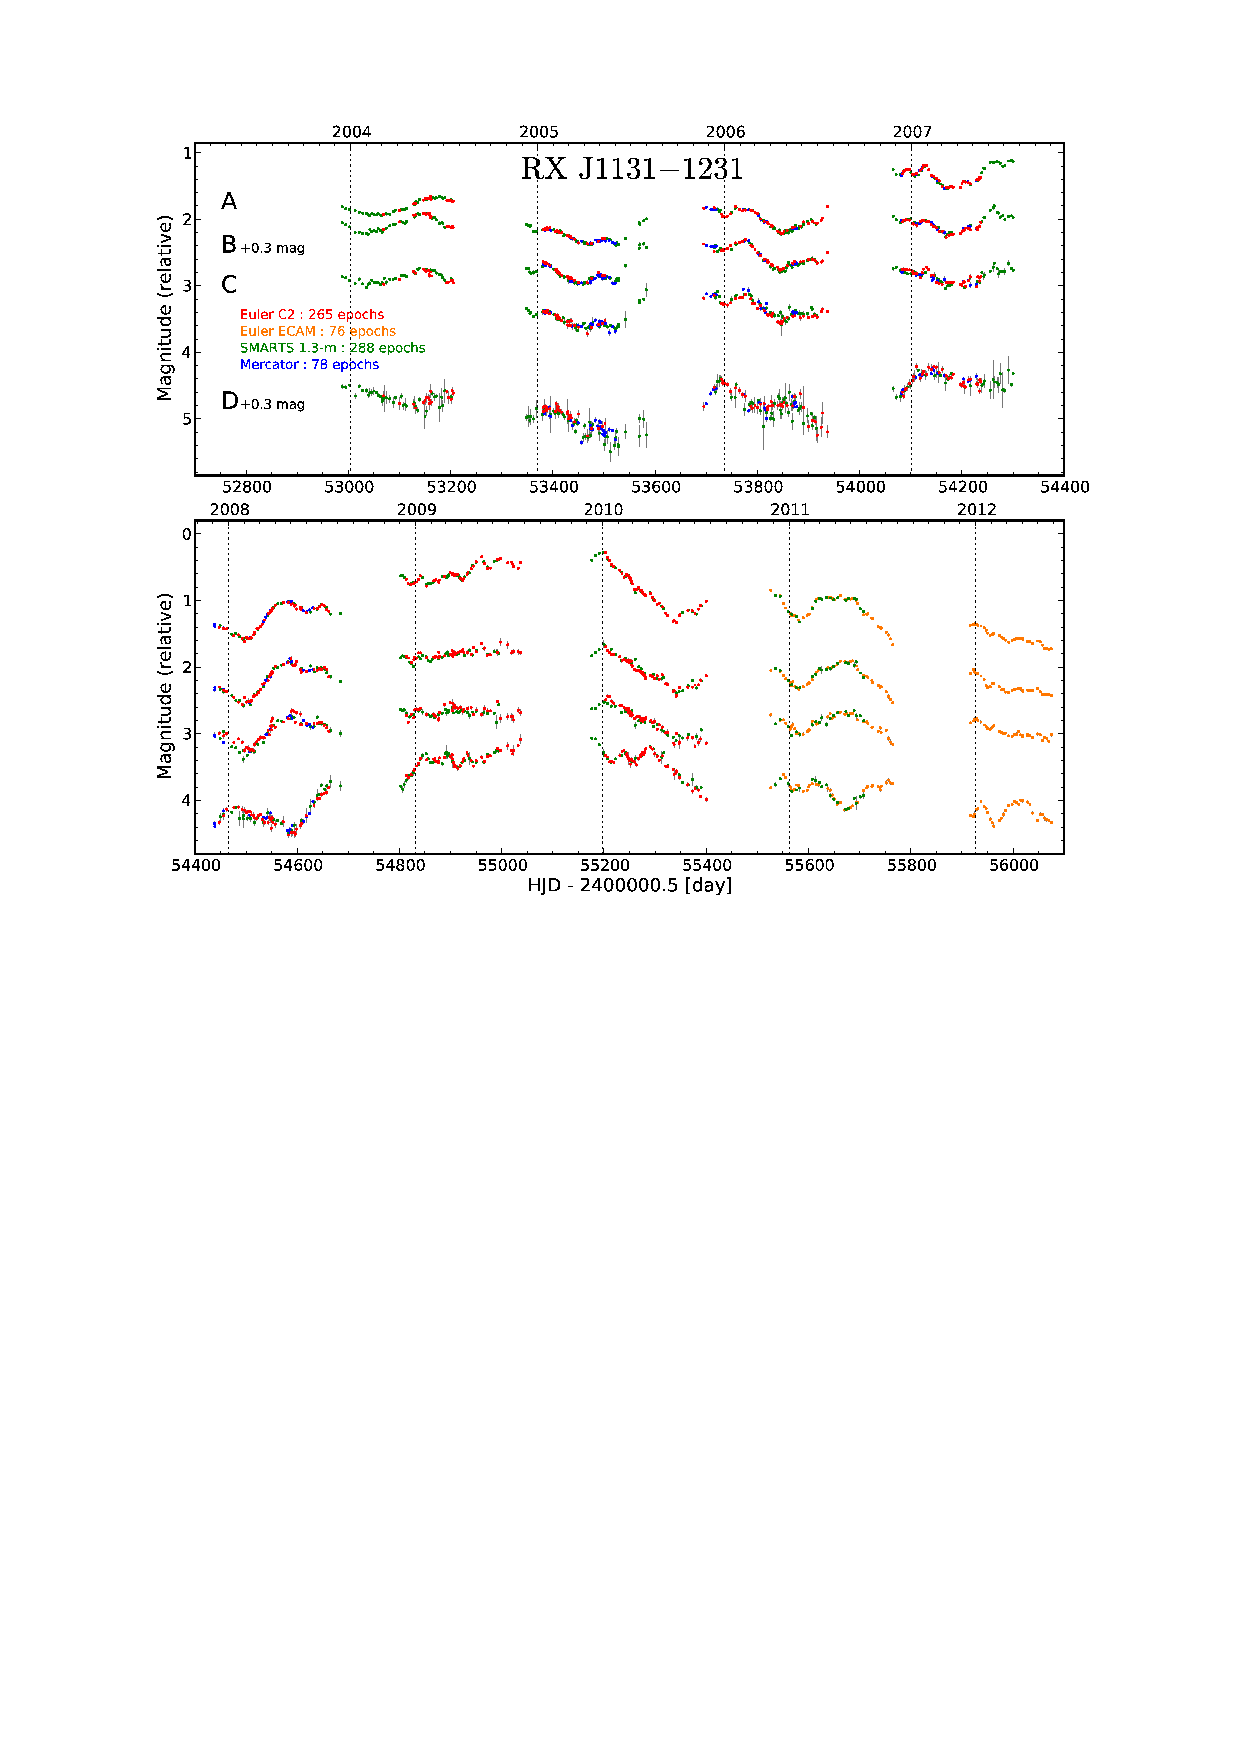
\includegraphics[width=0.48\textwidth]{figures/Tewes13-fig4.pdf}
\caption{Comparison between one of the early light curves \citep[left panel, from][]{Van89}, and a modern light curve from COSMOGRAIL \citep[right panel, from][]{Tew++13}. Note the improved photometric precision, cadence, and duration of the light curves, allowing for unambiguous determination of the time-delay to within 1-2\% precision.}
\label{fig:oldvsmoderndt}
\end{figure*}

Finally, when robust time delays started to become available, the
focus of the controversy shifted to the modeling of the gravitational
potential of the lens. Typically, in the mid ninenties, the only
constraints available to modelers were the quasar image positions and
to lesser extent flux ratios (limited by microlensing, variability and
differential extinction). Thus, the best one could do was to assume
some simple form for the lens potential like a singular isothermal
sphere \citep{K+F99}, thus breaking the mass sheet degeneracy, and to
neglect the effects of structure along the line of sight. Given these
necessary but oversimplistic assumptions, random errors grossly
underestimated the total uncertainty, leading to measurements
apparently inconsistent with those obtained by other groups or other
techniques
\citep{K+S04}. Since then, two methods have been pursued in order to
break degeneracies in more flexible modeling of the lensing data and
obtain realistic estimates on the uncertainties. One consists in using
large samples of systems with relatively weak priors
\citep{Ogu07b}. The other method consists in obtaining high quality data for
each lens system, such as detailed imaging of the quasar host galaxy
\citep{Keeton:2000p241,WBB04,Suy++06}, or non-lensing data like the deflector
stellar velocity dispersion \citep{T+K02b} and the properties of
galaxies along the line of sight \citep{K+Z04,Suy++10}. We discuss
these approaches in Section~\ref{ssec:lensmodel}. The astounding
improvement in data quality over the past two decades is illustrated
in Figure~\ref{fig:oldvsmodernimage}.

\begin{figure*}
\includegraphics[height=3.5cm]{figures/Schechter97_fg1.pdf}
\includegraphics[height=3.5cm]{figures/Suyu14_fig1.jpg}
\caption{Comparison between imaging data available in the nineties \citep[eft panel, from][]{Sch++97} and in the most recent studies \citep[middle and right panels, from][]{Suy++14}). With modern data the structure of the quasar host galaxy can be modeled in great detail, providing thousands of constraints on the deflection angle, and thus on the derivatives of the gravitational potential.}
\label{fig:oldvsmodernimage}
\end{figure*}

Ultimately, the controversies over systematic errors were essential to
spur the community to overcome the difficulties and find ways to
address them. This is a natural and probably inevitable part of the
scientific process. However, the bitterness of some of those
controversies during the ninenties and early naughts still resonates
today. Unfortunately, some of the scientists that followed the field
with excitement at that time, are still under the impression that
strong lensing time delays are inherently inaccurate and imprecise. As
we have briefly described here, and we will discuss in detail in the
next sections, in the last twenty years the field has moved forward
considerably implementing many solutions to the lessons learned the
hard way.


%%%%%%%%%%%%%%%%%%%%%%%%%%%%%%%%%%%%%%%%%%%%%%%%%%%%%%%%%%%%%%%%%%%%%%%%

\section{Theoretical background}
\label{sec:theory}

% Lensing, Fermat's principle and potential. Time delay surface.



\begin{figure*}
% \centering\includegraphics[width=0.96\textwidth]{figures/wavefront-schematic.pdf}
\caption{Schematic diagram, adapted from \citep{TreuAndEllis2015},
illustrating the origin of the gravitational time delay. The small
magnitude of the fractional  time delay (typically $\sim10$~days out of
$10^{12}$ days light travel time) is commensurate with the square of the
deflection angle (typically $\sim1$~arcsecond, or $\sim5\times10^{-6}$
radians).}
\label{fig:lineofsightcartoon}
\end{figure*}

% Time delay distance.

% Importance of mass distribution in lens.

% Model (mass-sheet) degeneracy and its generalizations

% Importance of mass along the line sight - the universe is not Friedmann Lemaitre Robertson Walker.


\begin{figure*}
% \centering\includegraphics[width=0.96\textwidth]{figures/line-of-sight-cartoon.pdf}
\caption{Cartoon illustration of line of sight effects in time delay
lens cosmography. Structures both within and outside the main lens
plane provide weak deflections to the light rays, affecting both the
image positions and time delays.} \label{fig:lineofsightcartoon}
\end{figure*}


%%%%%%%%%%%%%%%%%%%%%%%%%%%%%%%%%%%%%%%%%%%%%%%%%%%%%%%%%%%%%%%%%%%%%%%%

\section{Modern time delay distance measurement}
\label{sec:measurement}

Since 2010, it has been recognized that accurate cosmography with
individual lens systems involves the following key analysis steps.

\begin{description}
    \item{\bf Time Delay Estimation} The light curve extracted from
    monitoring observations is used as input to an inference of the
    time delay between the multiple images.
    \item{\bf Lens Modeling} High resolution imaging data are used to
    constrain a model for the lens mass distribution, which can be used
    to predict Fermat potential differences.
    \item{\bf Environment and Line of Sight Modeling} Additional observational
    information about the field of view around the lens system is used
    to account for the weak lensing effects due to massive structures in
    the lens plane and along the line of sight.
\end{description}

Cosmological parameter inference can then proceed -- although in
practice the  separation between this final step and the ones above is
not clean. Practitioners aspire to a joint inference of lens, source,
environment and cosmological parameters from all the data
simultaneously, but have to date broken the problem down  into the above
steps. In the next three sections we describe current state of the art,
limitations, and principal sources of systematic error of theses three
key measurement parts of the problem.

[WE MADE A NOTE TO ``MENTION IMPORTANCE OF BLINDNESS IN ALL
MEASUREMENTS'' -- BUT DO WE REALLY MEAN THIS?]


% % % % % % % % % % % % % % % % % % % % % % % % % % % % % % % % % % % %

\subsection{Measuring time delays}
\label{ssec:timedelay}

%Preamble.

Mention importance of blindness in all measurements.

%   %   %   %   %   %   %   %   %   %   %   %   %   %   %   %   %   %

\subsubsection{Monitoring Observations}

%State of the art: COSMOGRAIL optical monitoring.

%Limitations: scheduling.

%Systematic errors: uniform calibration and photometry.

Fassnacht for B1608
COSMOGRAIL.
Others?

%   %   %   %   %   %   %   %   %   %   %   %   %   %   %   %   %   %

\subsubsection{Lightcurve Analysis}

%State of the art: TDC results.

%Systematic errors: microlensing, correlated noise.

COSMOGRAIL
TDC


% % % % % % % % % % % % % % % % % % % % % % % % % % % % % % % % % % % %

\subsection{Modeling the lens mass distribution}
\label{ssec:lensmodel}

In addition to time delays, the second main ingredient entering the
determination of time delay distances is the mass model of the main
deflector. In the early days of time delay cosmography one could only
rely on the relative positions of the multiple images as constraints
(since in general the flux ratios are affected by micro and
millilensing, variability, and differential dust extinction, and are
therefore highly uncertain). Even for a quadruply imaged quasars, the
five positional constraints are insufficient to determine Fermat
potential differences to the desired level of precision and accuracy.

There are two classes of solution to the problem of underconstrained
lens models. One is to analyze large samples of lenses with physically
motivated priors and exploit the fact that cosmological parameters are
the same for all lenses to remove model degeneracies. A number of
attempts along these lines have been made \citep{Ogu07b,RK++2015}, and
it is easy to imagine that this solution will be popular in the
future, when large samples of lenses with measured time delays will be
available.

The alternative solution is to increase dramatically the number of
emprical constraints per lens system by means of dedicated high
resolution imaging and spectroscopic observations
\citep{Suy++10,Suy++13,Suy++14}. We describe this approach in detail
below.

For simplicity, in this section we describe only the case of a single
deflector in a single plane, leaving line of sight and environmental
effects for a later section. For clarity, we describe each step
corresponding to a different dataset individually. Ideally, all the
data, including the time delays, should be modeled holistically at the
same time---although in practice the problem has, to date, been broken up
into parts to make it more tractable.

%   %   %   %   %   %   %   %   %   %   %   %   %   %   %   %   %   %

\subsubsection{High resolution imaging observations}

Lensed quasars reside in a host galaxy. For typical redshifts of lens
and source, the host galaxy apparent size is of order
arcseconds. Images with sufficient depth and resolution to isolate the
bright point source and detect the lower surface brightness host
galaxy, often reveal extended lensed features connecting the
point-like images themselves (e.g. Figure~\ref{fig:oldvsmodernimage}).

In the best conditions these images cover hundreds if not thousands of
resolution elements. The distortion of the detailed features of the
lensed images are a direct measurement of the variation of the
deflection angle between the images.  In principle, for data with
infinite signal-to-noise ratio and resolution one could imagine
integrating the gradient of the deflection angle along a path between a
pair of images to obtain the difference in Fermat potential,
up to a mass sheet transformation (Section\ref{sec:theory}).
In practice, in the presence of noisy data and limited resolution,
forward modeling approaches have been the most successful so far, as
discussed below. From an observational point of view, it has been
demonstrated that images with $0.1''-0.2''$ FWHM resolution provide
good results, provided that the point spread function can be
appropriately modeled or reconstructed as part of the lens model
itself. The Hubble Space Telescope in the optical/near infrared
\citep{Suy++10,Suy++13,Suy++14,BirrerEtal2015} and the Very Large Baseline
Interferometer in the radio \citep{WBB04} have been the main sources
of images for this application. Recent progress in adaptive optics
imaging at the 10m W.M.~Keck \citep{Che++16}, the beautiful data being
obtained for lensed source by ALMA \citep{Hez++13a}, and the many
facilities currently being constructed or planned \citep{Men++15},
indicate that the prospects to scale up the number of systems with
available high resolution images are bright.

%   %   %   %   %   %   %   %   %   %   %   %   %   %   %   %   %   %

\subsubsection{Lens modeling techniques}

Conceptually, a detailed model of a lensed quasar and its host galaxy
needs to describe three different physical components: i) the surface
brightness of the source; ii) the surface brightness of the deflector;
iii) the gravitational potential of the deflector. It is useful to
conceptualize the problem in this way, in order to understand where
the information needed to break the degeneracy in the intrepretation
of the data comes from. Lensing is achromatic and preserves surface
brightness so any feature that belongs to the source \cite[including
in line of sight velocity][]{Hez++13} should appear in all the
multiple images (appropriately distorted). Likewise, the deflector is
typically a massive early-type galaxy with smooth surface brightness
distribution and approximately uniform colors \cite[except for dust,
see, e.g.][]{Suy++10}.

Each of the three components is typically described in terms of one or
both of the following choices:
i) simply parametrized functions such as a Sersic profile
for the surface brightness of the lens or the source, and a singular
isothermal ellipsoid for the gravitational potential of the deflector
\citep[e.g.][]{Mar++07,Kne++11,Kee11}; ii) as combinations of basis sets like surface brightness
pixels, lens potential pixel values, or Gauss-Hermite (``shapelet'')
functions
\citep[e.g.][]{Col08, BirrerEtal2015, Nig++15, TagoreAndJackson2016}. The latter class of
very flexible models require regularization to avoid overfitting the
noise in the data.\footnote{In the case of the shapelet basis set,
regularization can effectively be achieved through choosing the number of basis
functions to use as well as the scale of the underlying Gaussian. Most
analyses using shapelets having taken this approach to date, with
\citet{TagoreAndJackson2016} being a notable exception. A
promising alternative scheme would be to assign a less physically-motivated prior for the
shapelet coefficients.}
Hybrid approaches have been proposed where the parametrization of some of
the components is simple and others are complex
\citep{W+D03,T+K04,BrewerAndLewis2006,Suy++06}, or where flexibly-parametrized
``corrections'' are added to simply
parametrized models \citep{Koo05,V+K09,S+H10,Suy++10,BirrerEtal2015}.
The variety of
approaches in the literature reflect the inevitable tensions between
the need to impose as many physically motivated assumptions as
possible, while retaining sufficient flexibility to obtain a realistic
estimate of the uncertainties and avoid introducing biases by
asserting incorrect simplistic models. If the model is too constrained by the
assumption it will lead to underestimated errors, if it is more
flexible than necessary it will lead to a loss of precision.

Once the choice of modeling parametrization is set, exploring the
posterior PDF for the parameters is numerically non-trivial, often requiring weeks to months
of computing time. Fortunately, there are techniques to speed up the
calculations by limiting the number of non-linear parameters. For
example, for a given lens model, the transformation between source and
image plane can be described as a linear operation, or the pixellated
corrections to the potential can be found by linearizing the lens
equation (see references above).

Ideally, modeling choices should be explored systematically as well,
since they can potentially introduce systematic errors. This is
currently being done in the most advanced studies, at great expense in
term of computing time and investigator time. As we discuss in
Section~\ref{sec:outlook}, speeding up the modeling phase and reducing
the investigator time per system will be key to analyzing the large
statistical samples expected in the future.

%   %   %   %   %   %   %   %   %   %   %   %   %   %   %   %   %   %

\subsubsection{The role of stellar kinematics}

As introduced in Section~\ref{sec:theory}, stellar kinematics provide
a qualitatively different input and are therefore very valuable in
breaking degeneracies in the intepretation of lensing data
\citep[e.g., the mass-sheet degeneracy][]{Koo++03}, and in estimating systematic
uncertainties. Of course, translating kinematic data into estimates of
gravitational potential has its own uncertainties and degeneracies
(e.g. the mass anisotropy degeneracy for pressure supported systems),
but the combination of the two datasets in the context of a single
mass model has been proven to be very effective
\citep{T+K02a,T+K04}. Even a single measurement of stellar velocity dispersion,
interpreted via simple spherical Jeans modeling has been shown to
substantially reduce modeling uncertainties
\citep{T+K02b,Koo++03,Suy++14}. It is clear that getting spatially
resolved kinematic data will enable breaking the mass-anistropy
degeneracy \citep[see, e.g.,][and references therein]{Cou++14} and
thus better constraints on the lens model and thus of the resulting
cosmological inference (Agnello et al. 2016, in prep).


% % % % % % % % % % % % % % % % % % % % % % % % % % % % % % % % % % % %

\subsection{Lens environments and line of sight effects}
\label{ssec:los}

% State of the art: ray-traced cosmological simulations, matched via
% number counts.

% Limitations/systematics: incomplete model: local vs line of sight
% mass,  ignoring multi-plane lensing, external convergence only.

The analysis of B1608$+$656 by \citet{Suy++10} explicitly took into
account the weak lensing effects of external structures.  Such a
correction had been suggested by \citet{Fas++06b}, who identified 4
galaxy groups along the line of sight in a spectroscopic survey of the
B1608$+$656 field, and estimated that they could, if left unaccounted
for, bias any inferred Hubble constant high by around 5\%. Exactly how
to  model this effect has been the topic of a number of papers since
2010: the problem is  how to incorporate our knowledge of where the
galaxies are along the line of sight without introducing additional
bias due to the necessary assumptions about how their (dark) mass is
distributed, and how the rest of the mass budget in the field adds up.

\citet{Suy++10} attempted to solve these problems by comparing the
B1608$+$656 field with a large number of fields with similar  galaxy
number overdensity drawn from the Millenium Simulation, modeling the
line of sight effects with a single external convergence parameter and
accepting a somewhat broad prior distribution for it, in return for not
having to make  strong assumptions about the structure of the galaxy
groups in the field. The external convergence in the simulated fields
was calculated by ray-tracing by \citet{Hil++09}, and the
comparison in galaxy overdensity was enabled by the analysis of galaxy
number counts in archival HST images by \citet{FKW11}, who found that
the B1608$+$656 field was overdense by a factor of two. The resulting
prior PDF for the $\kappa_{\rm ext}$ parameter had median $0.10$ with
the 68\% credible interval spanning 0.05 to 0.18.


%%%%%%%%%%%%%%%%%%%%%%%%%%%%%%%%%%%%%%%%%%%%%%%%%%%%%%%%%%%%%%%%%%%%%%%%

\section{From time delay distances to cosmological parameters}
\label{sec:cosmo}

% Approach: combining CMB and time delay distances. Blinding.

% Results. Internal consistency. Consistency with other probes.

% Combination with stellar kinematics, introduces additional
% distance dependency. Not correlated, and weaker dependence than Ddt
% (See discussion with SHS about Jee et al papers)

Early approaches to inferring cosmological parameters from time delay
lens observations focused on measuring the Hubble constant in a
Friedman-Robertson-Walker model with asserted (fixed) density
parameters.\footnote{The original investigation by \citet{Ref64}
involved the ``assumption that the linear distance--red-shift relation
is valid.''} With better data came the recognition that time delay
lenses were really probes of cosmological distance
\citep{Koo++03,Suy++10}, and the emphasis shifted to
inferring the set of cosmological parameters that are needed  to predict
the kinematics of the expansion of the Universe out to the redshift of
the source.

The amount of cosmological information in an individual lens
is still relatively small, and the parameter most strongly constrained
is  the Hubble constant, but as sample sizes increase we expect
ensembles of  lenses to support the inference of several cosmological
parameters (or combinations thereof).

In Figure~\ref{fig:current-constraints} we reproduce the current best
constraints on  cosmological parameters, from the two best-measured
systems, B1608$+$656 and RXJ1131 \citep{Suy++14}. When this figure was
made, the available precision from just these two lenses was about the
same as that from SDSS DR7 BAO \citep{PercivalEtal2010} and the
``Constitution'' set of Type Ia supernovae \citep{HickenEtal2009}.
When all three of the curvature density $\Ok$, Dark Energy
density $\ODE$ and equation of state
$\wDE$ parameters are allowed to vary, along with $H_0$, we see that the
time delay lenses provide similar constraints to BAO and complementary
constraints to the SNe: the time delays and
the BAO signal depend on angular diameter distances and $H_0$, while
the supernovae probe luminosity distances.

%%%%%%%%%%%%%%%%%%%%%%%%%%%%%%%%%
\begin{figure*}[!ht]
\centering\includegraphics[width=0.9\linewidth]{figures/Suyu13_fig11.pdf}
\caption{Current cosmological parameter constraints from time delay
lenses. The marginalized posterior PDFs given the combined B1608$+$656
and RXJ1131 datasets and the assumption of an open CDM cosmology with
unknown dark energy equation of state is shown in
two sets of two parameter dimensions,
and compared to those given contemporary BAO and Type Ia supernova data.
Figure reproduced from \citet{Suy++14}.}
\label{fig:current-constraints}
\end{figure*}
%%%%%%%%%%%%%%%%%%%%%%%%%%%%%%%%%

While the sample of very well-measured lenses was being painstakingly
expanded from zero to two, the exploration of statistical approaches to
dealing with large samples of lenses began.  Compressing the image
configuration and time delay in double image systems into a single
summary statistic, \citet{Ogu07b} derived a scaleable  method for
measuring the Hubble constant (but not the other cosmological
parameters) from samples of lenses, finding
$H_0=68\pm6\,{\rm(stat.)}\,\pm8\,{\rm (syst.)}\,{\rm km s}^{-1}{\rm
Mpc}^{-1}$ from a sample of 16 lenses with measured time delays. The
systematic uncertainties associated with this result may be hard to
reduce given the approximations made: while the summary statistic is
model-independent, the  interpretation is not. An alternative approach
is to work with more flexible lens models, fit the data for each one,
and combine the whole sample in a joint inference.  This is the approach
taken by \citet{Sah++06}, who found  $72^{8}_{11}\,{\rm km s}^{-1}{\rm
Mpc}^{-1}$ from 10 lenses (again assuming fixed curvature and dark energy
parameters). With the  non-parametric (pixelated) mass
models used, the degeneracy between  density profile slope and predicted
time delay is broken by the choice  of pixel value prior PDF. This assumption was
tested by \citet{Rea++07}, who used a hydrodynamic simulation of an
elliptical galaxy to generate mock image position and time delay data,
and confirm the accuracy of the previous study's Hubble constant
uncertainties. With improved time delay estimates in a sample
of ten lenses, \citet{RK++2015} reduced the uncertainty to
$\pm6\,{\rm km s}^{-1}{\rm Mpc}^{-1}$. While focused only on the
Hubble constant, and with the lens environment and
line of sight mass structures remain unaccounted for and further tests
on realistic simulated galaxies warranted, these ensemble studies
point the way towards a future of considerably larger sample sizes.


%%%%%%%%%%%%%%%%%%%%%%%%%%%%%%%%%%%%%%%%%%%%%%%%%%%%%%%%%%%%%%%%%%%%%%%%

\section{Outlook}
\label{sec:outlook}

Motivation.

% % % % % % % % % % % % % % % % % % % % % % % % % % % % % % % % % % % %

% \subsection{Cosmic complementarity [TT]}
% PJM: I think this could function as the preamble for this section.
% We already have some mention of other probes in earlier sections,
% so it makes sense to motivate the forecasts in the next two subsections
% with the context being joint analysis. What do you think?

What's the point? Arent' other probes already doing it? Our place in the
cosmology ecosystem. Refer back to current constraints from \citet{Suy++13} in
Section~\ref{sec:cospars}, which show other probes.
Discuss place relative to other distance indicators
like Cepheids, BAO, Sne. Linder SL + SNe plots.

Then complementarity with growth of structure
probes like weak lensing, clusters etc etc. How important is H0?
Weinberg et al 2013, Kim et al 2014. Figure 48 from Weinberg?

Importance of multiple INDEPENDENT measurements for discovery of new
physics, and to ensure overall accuracy of cosmological parameters.
Define accuracy. Define precision. Segue.


% % % % % % % % % % % % % % % % % % % % % % % % % % % % % % % % % %

\subsection{Precision [PJM]}

With considerable observational and data analysis effort, the
feasibility  of reaching a precision  of 6-7\% in time delay distance
per lens has been demonstrated. The contributions to this error budget
from  the time delay measurement, mass model, and environment correction
are at present approximately equal and somewhat larger than the
estimated systematic errors. In this situation it makes sense to enlarge
the sample of lenses, in order to beat down the statistical
uncertainties. We return to the question of how to reduce the  residual
systematic errors in the next section.

\citet{C+M09b} made initial Fisher matrix forecasts of the likely
available precision on $H_0$ in large future surveys. They considered
several possible samples, concluding that 100 well-measured systems
(with 5\% distance precision each) should provide sub-percent precision
on the Hubble constant, and provide  dark energy parameter constraints
that are competitive with optimistic forecasts of other ``Stage IV''
cosmological probes. They also note that comparable constraints could be
available from a sample of 4000 time delay lens systems, each with only
photometric redshifts and simple image configuration model constraints
\citep[following][]{Ogu07b}.  Continued investigation of both samples
seems warranted, keeping in mind that the size of such a photometric
sample would be set by the availability of time delays measured at the
$\pm 2$~day level.

%%%%%%%%%%%%%%%%%%%%%%%%%%%%%%%%%
\begin{figure*}[!ht]
\centering\includegraphics[width=0.9\linewidth]{figures/Coe+Moustakas09_fig14.pdf}
\caption{Fisher matrix forecasts of cosmological parameters, based on
Dark Energy Task Force assumptions and having 5\% distance precision
for each of 100 time delay lenses. The Stage IV cosmological probes
being compared in an  open CDM cosmological model with time-variable
dark energy equation of state are weak lensing (WL), BAO, supernovae
(SN), cluster mass function (CL) and time delay cosmography (TD).
Figure reproduced from \citet{C+M09b}.}
\label{fig:fisher}
\end{figure*}
%%%%%%%%%%%%%%%%%%%%%%%%%%%%%%%%%

% Extrapolations to N lenses assuming X\% precision per time delay
% distance, forecasts.

% FIGURE: Forecasts for 10,50,100,1000 lenses for various cosmological
% models (w, wa+w0, curvature etc etc). CosmoSIS forecasts (ackn. Dave \&
% Elise, ask them).

What will it take to reach 5\% distance precision in each of 100 lenses?
If \citet{LiaoEtal2015} are right, this sized sample of lenses with
precise time delays should be able to be constructed from analysis of
the LSST light curves. The lens models for these systems should be able
to be constrained to sufficient precision using high resolution imaging
from next generation AO facilities, giant segmented mirror telescopes,
JWST and even WFIRST \citep{Men++15}. High overall mass model precision
will require good spectroscopic data as well: integral field units on
these same telescopes should be able to provide this. The contribution
to the distance uncertainty from the line of sight was particularly high
in the  cases of B1608 and RXJ1131: in most other systems in a large
sample the effects of the environment should be lesser, and they should
(effectively) average down \citep{Col++13}. The main challenge in
reaching the required Stage IV is likely to be the analysis cost: lens
modeling is something of a craft, and scaling up to large samples could
pose problems. Distributing the work among a large team of modelers will
be needed, an approach that is proving effective in the Frontier Fields
cluster lensing project \citep{FF}.

Note on approximation of forecasting using just Ddt,
and not DA as well: above plot is conservative.
Cite Jee et al paper 1 for pointing this out,
show figure from Jee et al paper 2?


% % % % % % % % % % % % % % % % % % % % % % % % % % % % % % % % % %

\subsection{Accuracy [PJM]}

Discussion of systematic uncertainties:

1) Time delay measurement. Light curve quality.

2) Lens mass modeling. Percent-level systematics due to model
assumptions (ie MSD). IFU observations, resolved stellar kinematics.
Ensembles.

3) Environment and line of sight

Other things: time delay perturbations (someone's noise is somebody else's signal..)
The importance of blinding.


%%%%%%%%%%%%%%%%%%%%%%%%%%%%%%%%%%%%%%%%%%%%%%%%%%%%%%%%%%%%%%%%%%%%%%%%

\section{Summary}
\label{sec:summary}

This review provides a succint review of gravitational time delays as
a tool for measuring cosmological parameters. In addition to giving a
brief introduction to theoretical underpinnings of the method, the
review discusses the past history of the field, before turning to
present day accomplishments and the challenges ahead. The main points
of this review can be summarized as follows:

\begin{enumerate}
\item From a theoretical point of view gravitational time delays are a clean and well understood probe of cosmic acceleration. Conceptually each time delay measurement provides a direct one step measurement of absolute distance. The typical redshifts of deflectors and sources span the range between $z\sim2$ and today, covering the cosmic time when dark energy arises to prominence.
\item Even though the potential cosmological application of strongly lensed time variable sources was recognized as early as 1964, it took decades for the method to come to fruition in practice. Two sets of challenges were overcome during the past two decades. Observationally, the main challenge was organizing long term monitoring campaigns and mustering the range of resources required to constrain accurate mass models. Theoretically, the main challenge consisted in learning how to exploit the available information to construct lens models with realistic estimate of the uncertainties.
\item Currently, it has been demonstrated through blind measurements that each individual system can deliver a measurement of absolute distance to about 6-7\%total uncertainty.  The power of the method is currently limited by the number of systems with well measured time delays and sufficient ancillary data to carry out detailed modeling ($\lesssim10$ at the time of this writing).
\item Two main ways forward are being pursued. On the one hand, systematic searches for strongly lensed quasars are under way and should be able to increase by 1-2 orders of magnitude the numbers of known suitable systems in the coming decade. With a relatively modest investment of follow-up telescope time, those samples will be sufficient to deliver measurements of cosmic acceleration that are competitive and highly complementary with other probes.
\end{enumerate}


it has been hard to put in practice for two reasons: multi-component
data and logistic considerations.

-Much progress has been made since 2000. Current precision. High
complementary with other probes

-Roadmap


Wise prophesy.


%%%%%%%%%%%%%%%%%%%%%%%%%%%%%%%%%%%%%%%%%%%%%%%%%%%%%%%%%%%%%%%%%%%%%%%%

%\paragraph{Paragraph headings} Use paragraph headings as needed.
%\begin{equation}
%a^2+b^2=c^2
%\end{equation}

% For one-column wide figures use
%\begin{figure}
% Use the relevant command to insert your figure file.
% For example, with the graphicx package use
%  \includegraphics{example.eps}
% figure caption is below the figure
%\caption{Please write your figure caption here}
%\label{fig:1}       % Give a unique label
%\end{figure}
%
% For two-column wide figures use
%\begin{figure*}
% Use the relevant command to insert your figure file.
% For example, with the graphicx package use
%  \includegraphics[width=0.75\textwidth]{example.eps}
% figure caption is below the figure
%\caption{Please write your figure caption here}
%\label{fig:2}       % Give a unique label
%\end{figure*}
%
% For tables use
%\begin{table}
% table caption is above the table
%\caption{Please write your table caption here}
%\label{tab:1}       % Give a unique label
% For LaTeX tables use
%\begin{tabular}{lll}
%\hline\noalign{\smallskip}
%first & second & third  \\
%\noalign{\smallskip}\hline\noalign{\smallskip}
%number & number & number \\
%number & number & number \\
%\noalign{\smallskip}\hline
%\end{tabular}
%\end{table}

%%%%%%%%%%%%%%%%%%%%%%%%%%%%%%%%%%%%%%%%%%%%%%%%%%%%%%%%%%%%%%%%%%%%%%%%

\begin{acknowledgements}
We are grateful to S.~Suyu and E.~Komatsu for insightful discussions
about the cosmological distance information content of time delay
lenses, and to S.~Suyu for making the B1608$+$656 MCMC chains
available for us to make Figure~\ref{fig:DdDdt}.
%
We thank S.~Birrer, V.~Bonvin, D.~Coe, T.~Collett, F.~Courbin, I.~Jee,
C.~Kochanek, E.~Linder, D.~Sluse and M. Tewes for very valuable feedback on a draft
of this review.
%
T.T. thanks the Packard Foundation for generous support through a
Packard Research Fellowship, the NSF for funding through NSF grant
AST-1450141, ``Collaborative Research: Accurate cosmology with strong
gravitational lens time delays''.
%
P.J.M. acknowledges support from the U.S.\ Department of Energy under
contract number DE-AC02-76SF00515.
\end{acknowledgements}

%%%%%%%%%%%%%%%%%%%%%%%%%%%%%%%%%%%%%%%%%%%%%%%%%%%%%%%%%%%%%%%%%%%%%%%%

% BibTeX users please use one of
\bibliographystyle{spbasic}      % basic style, author-year citations
% \bibliographystyle{spmpsci}      % mathematics and physical sciences
% \bibliographystyle{spphys}       % APS-like style for physics
\bibliography{references}   % name your BibTeX data base

% Non-BibTeX users please use
%\begin{thebibliography}{}
%
% and use \bibitem to create references. Consult the Instructions
% for authors for reference list style.
%
%\bibitem{RefJ}
% Format for Journal Reference
%Author, Article title, Journal, Volume, page numbers (year)
% Format for books
%\bibitem{RefB}
%Author, Book title, page numbers. Publisher, place (year)
% etc
%\end{thebibliography}

%%%%%%%%%%%%%%%%%%%%%%%%%%%%%%%%%%%%%%%%%%%%%%%%%%%%%%%%%%%%%%%%%%%%%%%%

\end{document}

%%%%%%%%%%%%%%%%%%%%%%%%%%%%%%%%%%%%%%%%%%%%%%%%%%%%%%%%%%%%%%%%%%%%%%%%
